\documentclass[12pt, a4pape]{article}
\usepackage[utf8]{inputenc}
\usepackage{fancyhdr}
\usepackage{multicol}
\usepackage[russian]{babel}
\usepackage{amsmath}
\usepackage{amssymb}
\usepackage[a4paper, margin=1in]{geometry}
\usepackage{graphicx}%Вставка картинок правильная
\usepackage{float}%"Плавающие" картинки
\usepackage{wrapfig}%Обтекание фигур (таблиц, картинок и прочего)
\usepackage[usenames]{color}
\usepackage{array}
\pagestyle{fancy}
\fancyhf{} % Очистка всех полей заголовков

% Установка номеров страниц
\fancyfoot[R]{\thepage} % Номер страницы справо


\setlength{\columnsep}{29pt}
\pagecolor[rgb]{0.996,0.949,0.827}
\geometry{
  a4paper,
  top=8mm, 
  right=16mm, 
  bottom=20mm, 
  left=8mm
}
\begin{document}
%\begin{center}
%\head{\LargeМАТЕМАТИЧЕСКИЙ КРУЖОК}
%\end{center}
\setcounter{page}{51}
\begin{figure}[H]

\centering

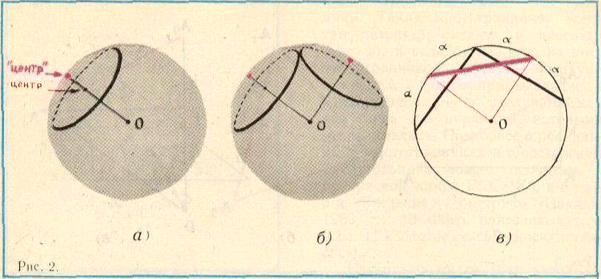
\includegraphics[width=1\linewidth]{picture.png}

\label{fig:mpr}

\end{figure}
\begin{multicols}{2}
Отсюда из леммы вытекает, что из чётных сомножителей можно огран\textit{ичиться только двойками, четв}ёркми и восьмёрками. Далее ясно, что \(2 \cdot 2\) хуже, чем \(4\), поскольку 
\[
(\left[\frac{2}{2}\right] + 1)^2 = 4 > \left[\frac{4}{2}\right] + 1 = 3. \hspace{0.4cm}\text{Выгодно}
\]
\(2 \cdot 4\) \textit{заменить} на 8, поскольку \(2 \cdot 3 = 6 > 5\); \(4 \cdot 4\) лучше, чем \(2 \cdot 8\), поскольку \(3 \cdot 3 = 9; 2 \cdot 5 = 10\) и, наконец, \(4 \cdot 4 \cdot 4 \text{ менее выгодно, чем } \(8 \cdot 8\)}, поскольку \(3 \cdot 3 \cdot 3 = 27;  \hspace{0.2cm}5 \cdot 5 = 25\), так что больше двух четвёрок оставлять нельзя. 

Итак, окончательный ответ такой: пусть \(N = 2^d p_1 \ldots p_m\), где \(m \geq 0, d \geq 0\) — целые, \(p_1, \ldots, p_m\) — нечётные простые числа. Обозначим произведение
\[
\frac{p_1 + 1}{2} \ldots \frac{p_m + 1}{2} \text{ через } P.
\]
\noident
Тогда наименьшее число сторонников Мирафлореса, достаточное для победы, равно
\\\\
$B_{} = 2\hspace{1mm}P, \text{ если } d = 1 \quad \text{(т.~е. } N = 2p_1 \ldots p_m \text{);}\\ B = 5^nP, \text{ если } d = 3n \hspace{1mm}\text{(} N = 8^n\hspace{1mm}p_1 \ldots p_m \text{);}\\B = 3 \cdot 5^nP, \text{ если } d = 3n+2 \hspace{1mm}\text{(}N=4 \cdot 8^np_1 \ldots p_m \text{);}\\B = 9 \cdot 5^nP, \text{ если } d = 3n+4 \hspace{1mm}\text{(}N=4^2 \cdot 8^np_1 \ldots p_m \text{);}\\\text{здесь n-целое число,}

Этот ответ нашли ученик 9-го класса из Томска \textit{А.~Гришков} и (в другой форме) ещё несколько читателей. В частности, для $N$ = 20 000 000 = 2^8 \cdot 5^7 = 4 \cdot 8^2 \cdot 5^7 \hspace{7mm}\text{получаем} \hspace{4mm} B = 3 \cdot 5^2 \cdot 3^7 = 164 \hspace{1mm} 025.

\columnbreak


\textbf{M2.} Дана сфера радиуса \(1\). На ней расположены равные окружности \gamma_0, \hspace{1mm} \gamma_1\text{,} \hspace{1mm} \ldots, \hspace{1mm} \gamma_n \text{ радиуса } \(r \hspace{1mm}(n\geq3)\). Окружность \gamma_0$ \hspace{1mm} касается всех окружностей  \gamma_1, \ldots, \gamma_n$; кроме того, касаются друг друга окружности  $\gamma_1$ и $\gamma_2; $ $\gamma_2$ и $\gamma_3; $ \ldots; $\gamma_n$ и $\gamma_1;  $

При каких $n$ это возможно? Вычислить соответствующий радиус \(r\).

\hspace{3mm}О т в е т: \(n = 3, 4, 5\).

\[
r = \sqrt{1-\frac{1}{4 \sin^2 \frac{\pi}{n}}}
\]

Каждой окружности на сфере можно сопоставить её <<центр на сфере>> — конец радиуса сферы, проходящего через центр окружности (никогда не лежащий на сфере). Эту точку мы будем называть <<центром>> окружности в кавычках, подчеркивающих, что это не <<обычный>> центр (рис. 2, $a$).

Заметим для точности, что такого определенного «центра» нет у окружностей двух больших кругов сферы, у которых центр совпадает с центром сферы. Но окружности, о которых идет речь в условии задачи, заведомо не могут иметь радиус 1, потому что окружности двух больших кругов не могут друг друга касаться, — они всегда пересекают друг друга в двух диаметрально противоположных точках сферы. 

Точка касания двух окружностей, расположенных на сфере (см. рис. 2, $б$), лежит в плоскости $p$, проходя-
\end{multicols}
\newpage
\setcounter{page}{49}


\begin{center}
\renewcommand{\arraystretch}{0.7}
\setlength{\tabcolsep}{3pt}
\begin{tabular}{l c c c c ccccc}
\hline
Ранг группы $r$ & 1 & 2 & 3 & 4 & 5 & 6 & 7 & 8 & 9 \\
Общее число групп ранга $r$ & $5$ & $5^2$ & $5^3$ & $5^4$ & $5^5$ & $5^6$ & $5^7$ & $2^4\cdot5^7$ & $2^8\cdot5^7$ \\
Сколько из них чёрных & 3 & $3^2$ & $3^3$ & $3^4$ & $3^5$ & $3^6$ & $3^7$ & $3^9$ & $3^{11}$ \\ 
Сколько человек в одной груп- & $4 \cdot 10^6$ & $8 \cdot 10^5$ & $16 \cdot 10^4$ & $32 \cdot 10^3$ & $64 \cdot 10^2$ & 1280 & 256 & 16 & 1 \\ 
пе ранга $r$ \\
На сколько групп ранга $(r+1)$ & 5 & 5 & 5 & 5 & 5 & 5 & 16 & 16 & - \\ 
разбивается каждая группа ран-\\
га $r$ \\
Сколько чёрных подгрупп ран- & 3 & 3 & 3 & 3 & 3 & 3 & 9 & 9 & - \\
га $(r+1)$ у чёрной группы ран-\\
га $r$ \\ \hline
\end{tabular}
\end{center}


\end{document}
